\documentclass[../tp2_grupo404.tex]{subfiles}

\graphicspath{{\subfix{../out/}}}

\begin{document}

\subsubsection{Criterio de selección}

En el enunciado nos pide que el programa sirva para, con respecto a una nueva fábrica,
\textquote{determinar dónde la ubicarán para minimizar los gastos de logística y distribución}.
Pero también se indica que: \textquote{Cada ruta une dos depósitos en un
sentido. No todos los depósitos tienen rutas que los conecten}.

Así mismo se indica que se debe emplear el algoritmo de Johnson; éste
pruduce una tabla de distancias. Sin embargo, para emplearlo a tal fin es
necesario tomar una serie de decisiones relevantes para el criterio de selección,
a saber:
\begin{enumerate}
    \item Si todos los depósitos cuentan con la misma improtancia o si existe
    alguna ponderación.
    \item Con las condiciones dadas es posible encontrarse con la disyuntiva de
    acceder a pocos depósitos pero con mejor costo (incluso negativo) o elegir
    una opción con un costo más alto pero con acceso a más depósitos (aunque aun
    así no a todas).
\end{enumerate}

Para el primer punto, hemos asumido que todos cuentan con la misma importancia;
de lo contrario suponemos que se nos hubiera indicado que también se provee
una tabla de ponderaciones.

En cambio para el segundo entendemos que siendo una decisión con un posible
impacto considerable y que dependa de circunstancias más allá del modelo actual
(o, incluso, muy difíciles de modelar), le brindamos la información al usuario
para que tome la decisión con el criterio que considere preferibel.

Mientras que si hay al menos un vértice que llegue al máximo de nodos con el
mínimo costo, se tomará como la mejor recomendación (a pesar de que puedan
existir otros nodos con el mismo costo pero menos alcance o el mismo alcance
con mayor costo).

\begin{figure}[H]
    \centering
    \subcaptionbox
        {\label{grafoDisyuntiva}\textbf{Grafo de ejemplo que nos llevaría a la disyuntiva}}
        {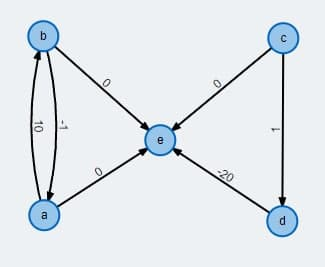
\includegraphics[width=0.4\linewidth,angle=0,origin=c]{img/disyuntiva.jpg}}
    \subcaptionbox
        {\label{outDisyuntiva}\textbf{Salida del programa, con y sin disyuntiva.}}
        {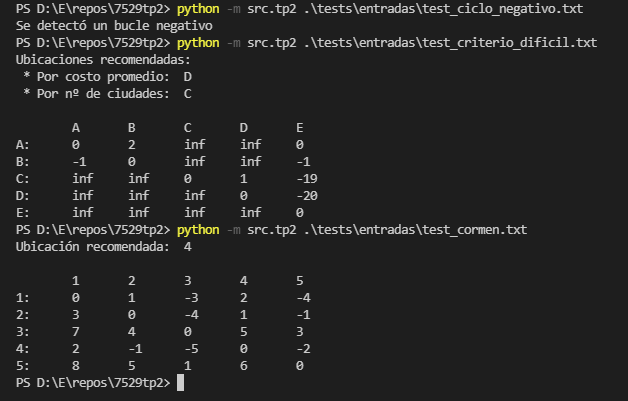
\includegraphics[width=0.4\linewidth,angle=0,origin=c]{img/salida.jpg}}
\end{figure}

Por ejemplo, para el caso del \cref{grafoDisyuntiva} si la fábrica se ubicara en
D tendría un costo promedio de -20 (es decir, genera ganancia), pero acceso a un sólo
depósito adicional; y si se ubica en C tiene un costo de -18, pero no puede alcanzar
a C ni D.

Entonces, será un usuario más conocdedor del problema quien podrá decidir si alguna de
las dos es una situación aceptable y cuál es preferible (¿cuál es el costo de no acceder
a ciertos depósitos?), o si sería preferible posponer la construcción de la fábrica y,
en ese caso, qué acciones se deben tomar; tales como crear una ruta, etc.

% FIN DEL DOCUMENTO (SECCIÓN P1.7)
% NO BORRAR POR ACCIDENTE NI ESCRIBIR COSSA ABAJO
\end{document}
